\chapter{Phương pháp đề xuất}
\label{Chapter3}

Trong chương này, chúng tôi tổng hợp và cài đặt một mô hình giúp trích xuất thông tin tên thuốc từ ảnh, đặt tên là \codeword{MEP}. Đầu vào của mô hình là đơn thuốc, được biểu diễn dưới dạng ảnh. Chúng tôi thực hiện tiền xử lý ảnh sau đó đưa đến CRAFT. CRAFT như đã đề cập tại \cite{baek2019character}, sẽ giúp khoanh vùng các khu vực trên ảnh nơi có thể chứa văn bản. Ưu điểm của CRAFT là nó hỗ trợ khoanh vùng các văn bản theo cấp độ thấp nhất, cấp độ theo từng từ, từ đó sẽ khắc phục được phần lớn các vấn đề liên quan đến ảnh đầu vào ví dụ như bị nghiêng, mờ, lệch,... Các vùng đó sẽ được cắt ra độc lập và đưa đến VietOCR \cite{VietOCR} nhằm mục đích chuyển đổi nó trở thành văn bản. VietOCR là một mô hình mới, hỗ trợ tiếng Anh cũng như rất tốt cho tiếng Việt, giúp hiệu quả của bước nhận dạng đạt tối đa cho các hoá đơn đơn thuốc có chứa nhiều từ tiếng Việt. Bên cạnh đó, chúng tôi cũng xây dựng một thuật toán đặc biệt giúp gom nhóm các từ trên cùng một dòng vào thành một câu, từ đó giúp xây dựng ngữ cảnh của câu một cách rõ ràng trước khi chuyển đến những bước tiếp theo. Tại đây, toàn bộ văn bản được biểu diễn dưới dạng ảnh trong hình ảnh đơn thuốc đã được chuyển đổi thành văn bản mà máy tính và các hệ thống phía sau có thể hiểu được.

Khác với mô hình trước đó, thay vì lấy toàn bộ kết quả của bước OCR ra để so sánh với từ điển thuốc, chúng tôi lựa chọn một con đường khác, trước tiên trích xuất các từ hay cụm từ nằm ở vị trí có thể là tên thuốc trong câu, sau đó kiểm tra chéo với một mô hình tên là Medicine Classifier với nhiệm vụ phân loại tập từ là thuốc ra khỏi tập dữ liệu nhiễu kể trên. Kết quả của bước này là đã ổn định, chỉ cần đưa vào một phần cuối cùng đó là sửa lỗi bằng cách so khớp các tên thuốc đã nhận dạng được với hệ thống từ điển tên thuốc để cho ra kết quả cuối cùng.

Sau đây khoá luận sẽ đi lần lượt qua các phần trong phương pháp đề xuất để làm rõ hơn mục đích và công dụng của các bước trong việc trích xuất thông tin thuốc ra khỏi đơn thuốc. Hình ~\ref{fig_proposed} mô tả lại một cách khái quát các thành phần trong \codeword{MEP}.

\begin{figure}
\centering
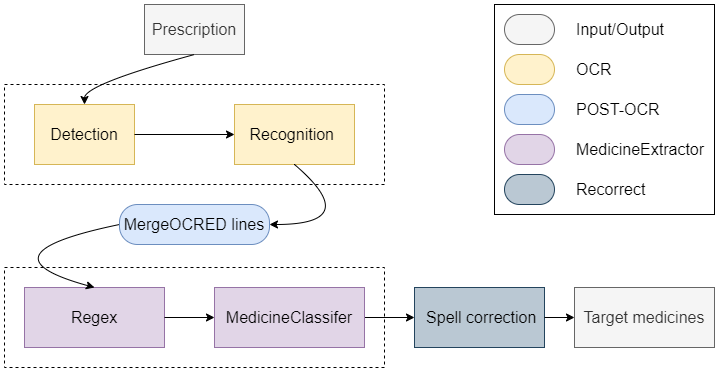
\includegraphics[width=0.9\textwidth]{mep_img/proposed_method.png}
\caption{Cấu trúc của mô hình đề xuất (MEP)}\label{fig_proposed}
\end{figure}

\section{OCR}

Trong phần OCR này, mục tiêu quan trọng cần phải làm là chuyển đổi các ảnh đầu vào thành văn bản mà máy tính có thể hiểu được. Các ảnh đầu vào thường rất đa dạng về cả kiểu dáng, cũng như nội dung. Một ảnh đơn thuốc do người dùng chụp lại đôi khi có thể dựng đứng, đôi khi thì nằm ngang, thậm chí là bị nghiêng dẫn đến cần một thuật toán đủ tốt để trích xuất được văn bản bên trong. Khoá luận sẽ khai thác 2 thành phần trong bước OCR, đó là phát hiện văn bản (Text Detection) và nhận dạng văn bản (Text recognition).

\subsection{Phát hiện văn bản bằng CRAFT}

Chúng tôi lựa chọn CRAFT cho việc phát hiện văn bản dựa trên cách hoạt động của nó. CTPN \cite{tian2016detecting} là một thuật toán phát hiện văn bản tốt, cho phản hồi nhanh tuy nhiên nó không đạt được kết quả ấn tượng đối với đa số ảnh đơn thuốc. Điều đó là do liên quan đến tính chất của phương pháp phát hiện. CRAFT có thể phát hiện từng từ độc lập trong một câu bất kì, trong khi CTPN chú trọng thêm cả vào ngữ cảnh của câu và phát hiện cả dòng tại một thời điểm.

Đối với các hình ảnh đơn thuốc khó phát hiện, ví dụ như bị nghiêng, bị mờ, bị nhiễu hoặc đơn giản là các từ quan trọng trong câu bị che đi, CTPN sẽ bộc lộ rõ nhược điểm rằng trả ra các kết quả nhận dạng không thực sự đúng, không đáp ứng được nhu cầu hiện tại. Ngược lại, dựa trên các bounding box thu thập được từ CRAFT, ta hoàn toàn có thể xây dựng lại cấu trúc câu để đảm bảo ngữ nghĩa cho văn bản được trích xuất nếu cần. Hình ~\ref{fig_craft_pres_2} và ~\ref{fig_craft_pres_1} thể hiện kết quả của CRAFT trên một đơn thuốc cụ thể. 

\begin{figure}
\centering
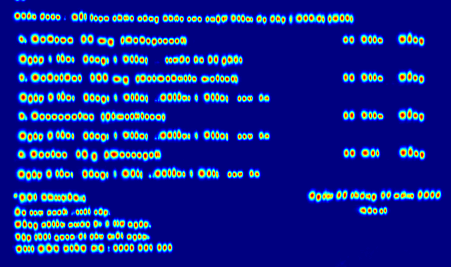
\includegraphics[width=0.9\textwidth]{mep_img/craft_pres_2.png}
\caption{CRAFT phát hiện các thông tin văn bản trong đơn thuốc.}\label{fig_craft_pres_2}
\end{figure}

\begin{figure}
\centering
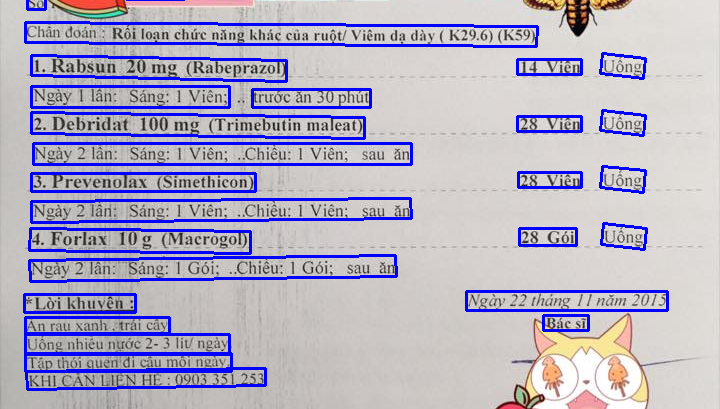
\includegraphics[width=0.9\textwidth]{mep_img/craft_pres_1.png}
\caption{Kết quả phát hiện văn bản của CRAFT trong đơn thuốc sau khi được đóng bounding box.}\label{fig_craft_pres_1}
\end{figure}

\subsection{Nhận dạng văn bản sử dụng VietOCR}

VietOCR \cite{VietOCR} là một mô hình nhận dạng văn bản, chữ viết có hỗ trợ tiếng Việt và đồng thời được người Việt phát triển. Tác giả của VietOCR giới thiệu 2 kiểu cài đặt mô hình, một là Transformers, hai là Sequence-to-sequence (Seq2Seq). Cả 2 hướng cài đặt đều cho ra kết quả tốt, tuy nhiên Transformers hiện đại hơn nhưng lại không có nhiều sự khác biệt về độ chính xác tốt hơn. Vì vậy chúng tôi lựa chọn theo hướng Seq2Seq nhằm tiết kiệm chi phí về mặt thời gian nhận dạng. 

Cách hoạt động của VietOCR đó là nhận dạng theo từng dòng, từ đó chúng tôi có thể sử dụng ngay kết quả trả về của bước phát hiện văn bản bằng CRAFT phía trên làm đầu vào cho VietOCR, mỗi vùng phát hiện văn bản sẽ được nhận dạng và chuyển đổi về văn bản tương ứng. Kết quả của VietOCR sẽ là toàn bộ văn bản trong đơn thuốc.

\section{Medicine Extractor}

Sau khi trải qua bước OCR, chúng ta đã có được toàn bộ văn bản của đơn thuốc. Thông thường, các phương pháp truyền thống sẽ lấy tất cả các văn bản này đưa vào so khớp với một kho dữ liệu gồm từ điển tên thuốc nhằm lọc ra những tên thuốc đúng. Tuy nhiên, kích thước của một bộ từ điển tên thuốc đầy đủ, có chứa đa số tên thuốc hiện đang được lưu hành có kích thước không hề nhỏ. Nếu như ta lấy tất cả văn bản để so sánh thì chi phí so khớp sẽ bị nhân lên gấp nhiều lần. Để khắc phục trường hợp đó, chúng tôi đề xuất một bước bổ sung nhằm cố gắng tối đa lọc ra những cụm từ có khả năng là tên thuốc nhất có thể sao cho vẫn đảm bảo hiệu quả mô hình đồng thời giảm số bước so sánh thêm sau này.

Trong đơn thuốc, ngoài tên thuốc ra thì ta cũng bắt gặp nhiều thông tin khác có thể kể đến như là thông tin bệnh nhân, thông tin cơ sở cấp thuốc, chuẩn đoán bệnh, liều lượng, nguyên liệu, cách sử dụng... Nếu như ta có thể bỏ bớt các thông tin này trước khi so khớp với từ điển thì sẽ cho ra hiệu suất mô hình đạt tốt hơn nhiều so với cách làm cũ.

\begin{figure}
\centering
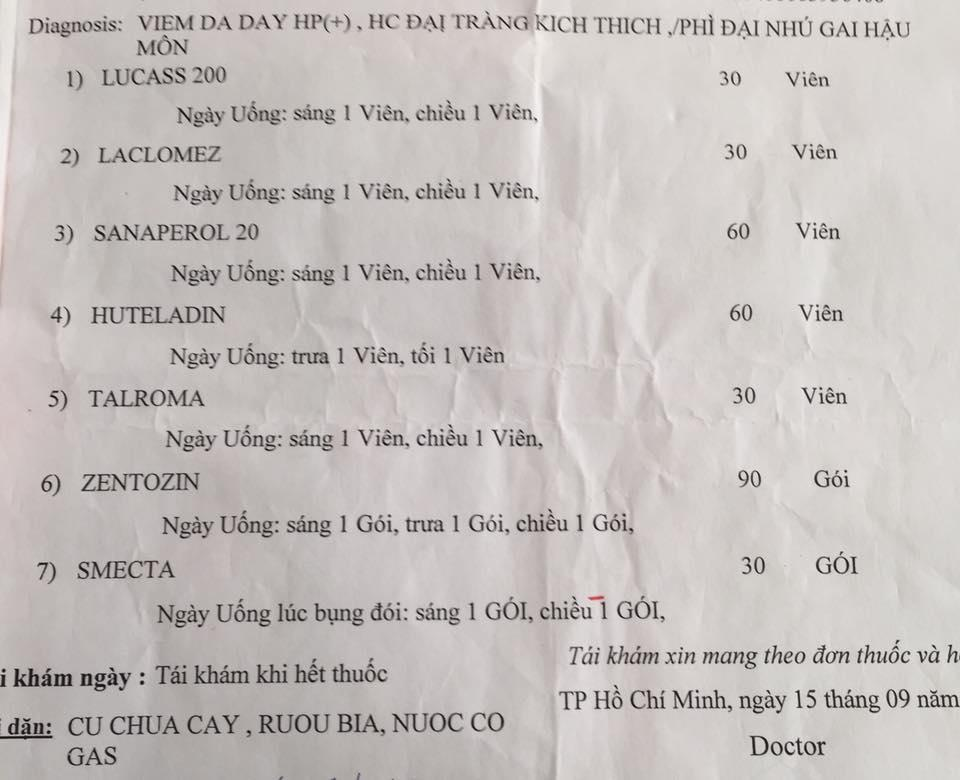
\includegraphics[width=0.7\textwidth]{mep_img/med_extr.png}
\caption{Ví dụ về đơn thuốc, với nội dung bên trong thông thường đều theo một bố cục với quy luật nhất định. Các tên thuốc được liệt kê theo từng hàng, từ trên xuống dưới, với bên trái đang được đánh số thứ tự.}\label{med_extr}
\end{figure}

Thông thường, đơn thuốc cũng giống như các loại hóa đơn, đó chính là bố cục của đơn thuốc sẽ tuân theo một cấu trúc hoặc bán cấu trúc nào đó. Danh sách các tên thuốc trong một đơn thường được trình bày theo một trình tự cố định nhằm giúp bệnh nhân và bác sĩ quan sát dễ hơn. Hình ~\ref{med_expr} biểu diễn một mẫu đơn thuốc cụ thể. Vì thế ta có thể dựa vào mẫu này để trích xuất các từ hay cụm từ có khả năng cao là tên thuốc ra khỏi tập ban đầu bằng các luật (heuristic rules), chúng tôi gói gọn tập luật này vào trong một bước gọi là \textbf{Medicine Extractor}.

Nhờ vào quan sát trên, ta có thể phân loại các đơn thuốc ra làm hai nhóm chính, sau đó tiến hành tách tên thuốc tiềm năng ra khỏi đơn thuốc thông qua một tập các Regular Expression:


\begin{itemize}

\item[-] Luật 01. \textbf{^([0-9]+)(?:\textbackslash.|\textbackslash,)* *(?:(.*?) *\textbackslash((.*?)\textbackslash)*|(.*?) *\\\textbackslash((.*)|(.*)|(\textbackslash(.*?\textbackslash)))}. Theo trường hợp này, mỗi tên thuốc sẽ nằm trên một dòng và có số thứ tự đứng trước. Trên dòng đó, ngoài tên thuốc thì cũng đi kèm với hoạt chất nằm chung (vị trí của tên thuốc và hoạt chất có thể hoán đổi cho nhau tùy đơn thuốc, tuy nhiên vẫn đảm bảo thành phần liền sau sẽ nằm trong dấu ngoặc đơn. Với luật này, ta có thể trích xuất được một lượng tối thiểu các tên thuốc ra khỏi đơn thuốc, đồng thời khả năng chúng là tên thuốc cũng cao nhất, vì hầu hết chỉ dòng chứa tên thuốc mới có nhu cầu có số đứng trước. Hình ~\ref{med_extr_rule_1} chỉ ra một mẫu đơn thuốc thuộc luật 1.

\begin{figure}
\centering
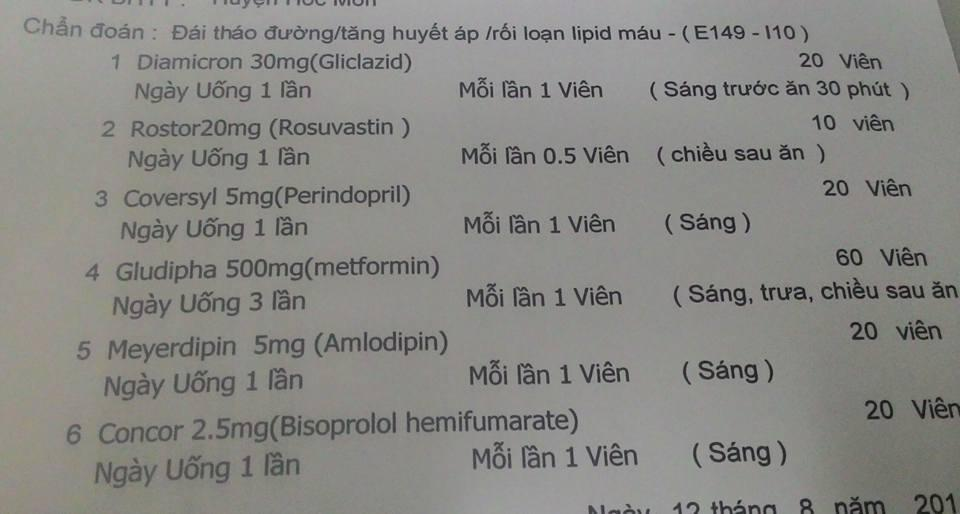
\includegraphics[width=0.8\textwidth]{mep_img/med_extr_rule_1.png}
\caption{Mẫu đơn thuốc có dạng như luật 01 đề cập khi dùng Medicine Extractor.}\label{med_extr_rule_1}
\end{figure}

\item[-] Luật 02. \textbf{^(?:(?!(?:\textbackslash(| ))(.+?) *\textbackslash(+([^)\textbackslash n\textbackslash r]+)\textbackslash)*)}. Luật này cũng tương tự như luật đầu tiên, tuy nhiên bỏ bớt đi điều hiện là phải có số đứng trước. Bằng cách này, ta có thể xử lý được thêm cả những dòng chứa thuốc mà không có số thứ tự. Luật này tuy sẽ làm tăng số dòng nhận được, tuy nhiên vẫn sẽ đảm bảo hiệu suất mô hình, đồng thời là bước dự phòng khi OCR vì vấn đề nào đó mà không thể nhận diện được số thứ tự đứng trước tên thuốc. Hình ~\ref{med_extr_rule_2} đề cập đến một ví dụ cho trường hợp đơn thuốc tuân theo luật 2.

\begin{figure}
\centering
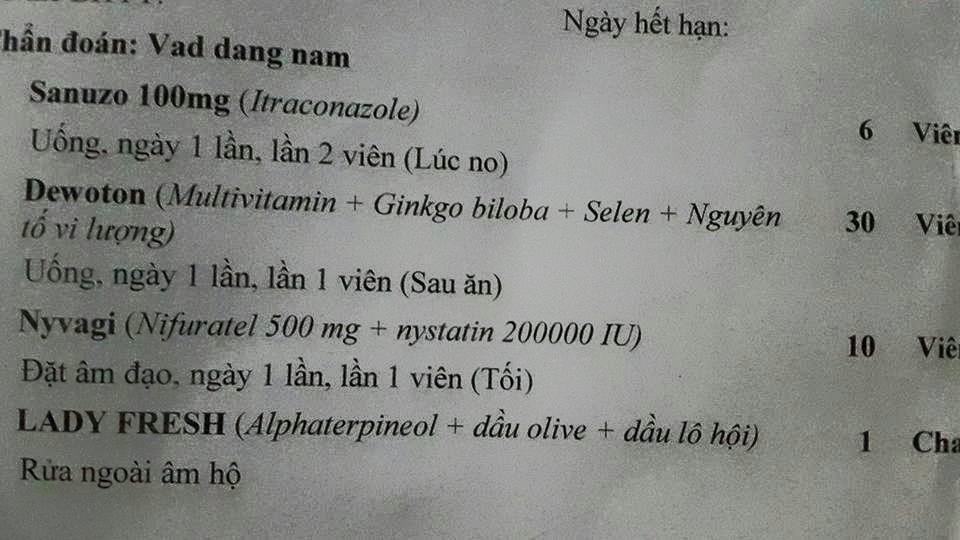
\includegraphics[width=0.7\textwidth]{mep_img/med_extr_rule_2.png}
\caption{Mẫu đơn thuốc có dạng như luật 02, không có số thứ tự đứng đầu.}\label{med_extr_rule_2}
\end{figure}

\item[-] Ngoài ra, có một số ít mẫu đơn thuốc có dạng tên thuốc và hoạt chất nằm trên nhiều dòng. Tuy nhiên trường hợp này ít xảy ra nên khóa luận không tập trung vào để đảm bảo hiệu năng của mô hình. Hình ~\ref{med_extr_rule_3} thể hiện một trường hợp rõ nét nhất cho một đơn thuốc không thuộc phạm vi quản lý của \codeword{MEP}.

\begin{figure}
\centering
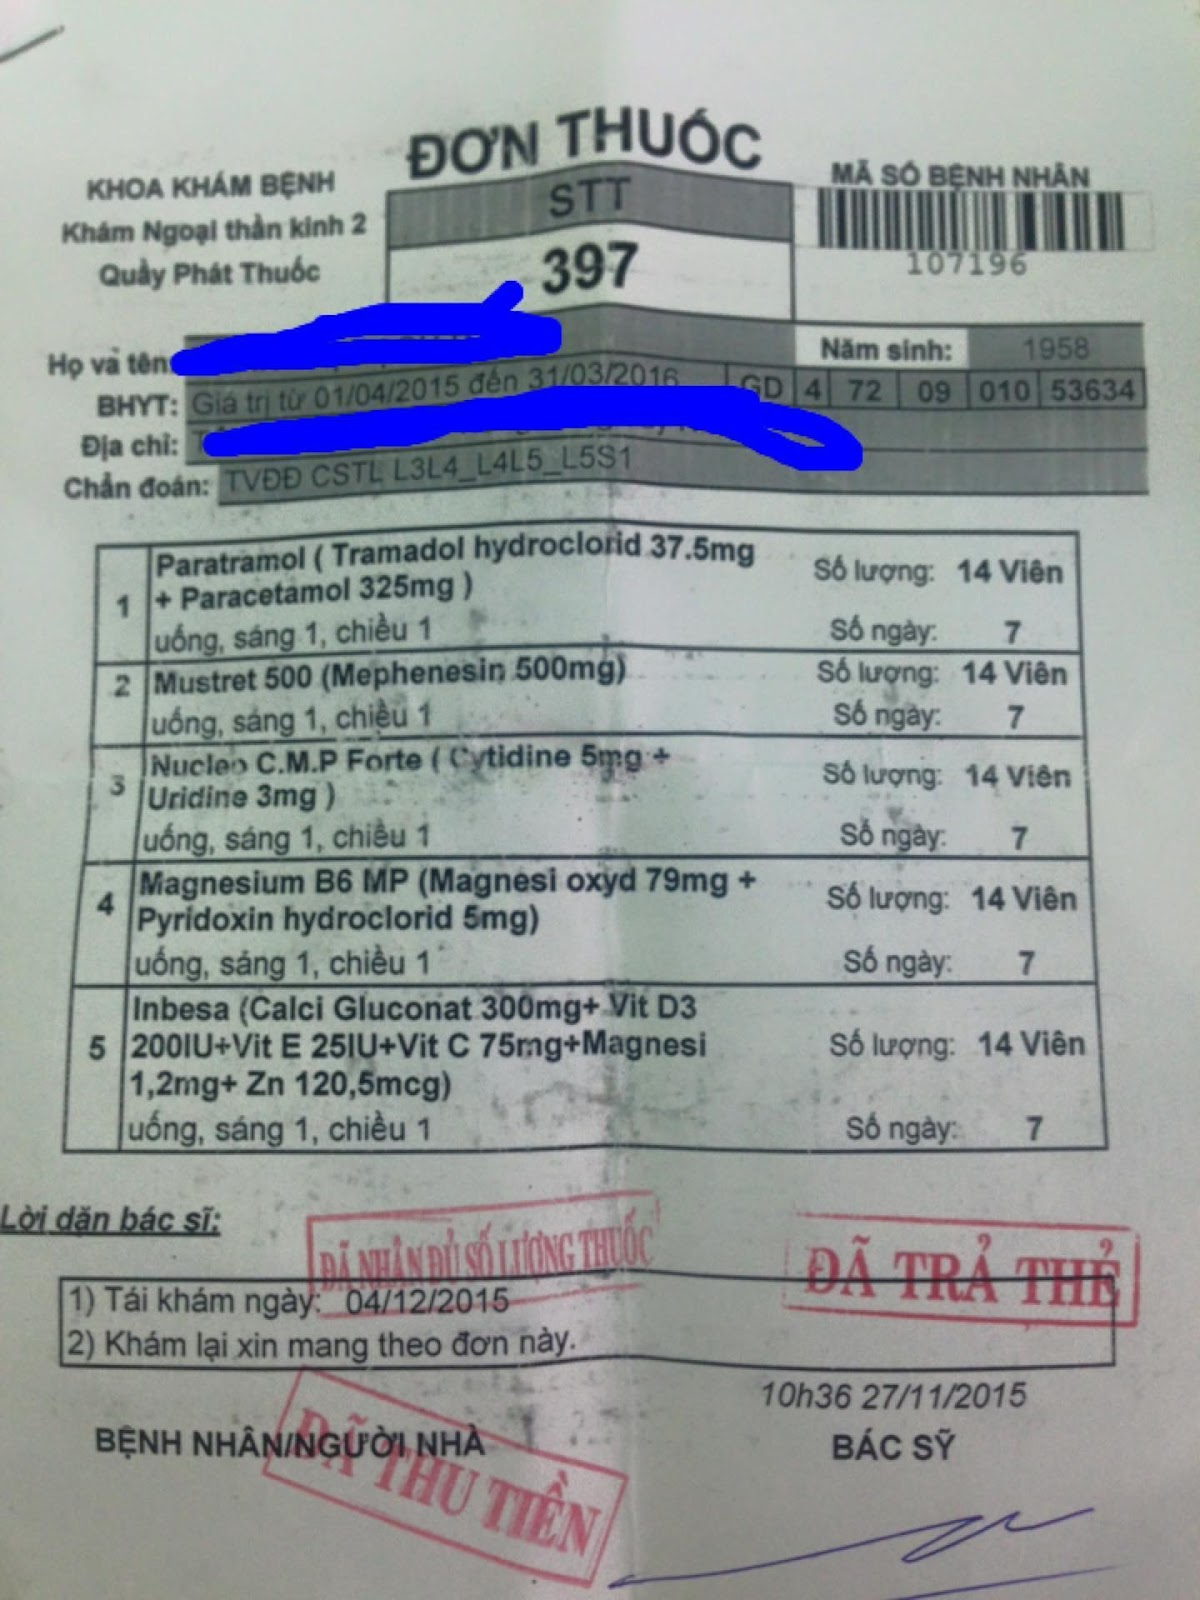
\includegraphics[width=0.7\textwidth]{mep_img/med_extr_rule_3.png}
\caption{Mẫu đơn thuốc không có dạng đặc biệt, khi tên thuốc và hoạt chất nằm trên cùng một dòng nhưng giao diện in lại có cắt dòng dẫn đến có thể có 2 dòng cho mỗi dòng thuốc.}\label{med_extr_rule_3}
\end{figure}

\end{itemize}

\section{MergeOCR}

Để việc trích xuất dựa trên Regex hoạt động tốt, các dòng chứa tên thuốc cần được phát hiện và đóng khung đầy đủ các thành phần cần thiết. Tuy nhiên, do hình ảnh có thể bị mờ, nhiễu khiến cho thuật toán OCR có thể không thực hiện tốt. Nghĩa là thay vì các vùng phát hiện được kỳ vọng chứa tất cả chữ số, tên thuốc và thành phần thuốc thì kết quả nhận được là tập hợp nhiều bounding box chứa các thành phần riêng lẻ giống như trong hình ~\ref{mergeocr_1}. Hậu quả là hệ thống Medicine Extractor được mô tả phía trên sẽ không thực hiện được hiệu quả do không khớp với biểu thức RegEx.

Nhằm khắc phục vấn đề, chúng tôi đề xuất một bước mở rộng tên là MergeOCR. Mục đích của bước này là tìm cách gom các văn bản của các bounding box trên cùng một dòng thành một dòng văn bản duy nhất. Ngoài việc một dòng bị tách thành các bounding box khác nhau, chúng tôi còn gặp phải vấn đề là ranh giới giữa các bounding box này có thể không tách biệt rõ ràng. Trong một vài trường hợp, các khung được phát hiện trong hình ảnh đơn thuốc nằm chồng chéo lên nhau, dẫn đến ta hay lầm tưởng rằng chúng đang nằm cùng trên một dòng. Vì thế, thuật toán đề xuất cần cải thiện tốt cả hai khía cạnh này.

\begin{figure}
\centering
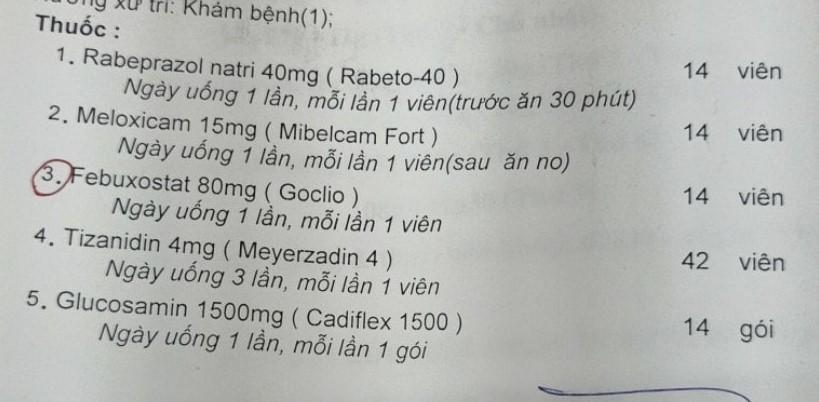
\includegraphics[width=0.7\textwidth]{mep_img/mergeocr_1.png}
\caption{Mẫu đơn thuốc bị méo khiến cho các bounding box của bước phát hiện văn bản bị chồng chất lên nhau, không được coi là một hàng độc lập.}\label{mergeocr_1}
\end{figure}

Chúng tôi đề xuất sử dụng thuật toán Agglomerative Hierarchical Clustering (AHC) cho việc gom nhóm các khung trên cùng một dòng về lại thành một nhóm duy nhất. Thuật toán AHC có ưu điểm là đơn giản, không cần xác định trước số nhóm cần gom cụm. Trong trường hợp này, ban đầu tất cả các bounding box sẽ được đưa vào một nhóm riêng tương ứng. Sau đó thuật toán sẽ lặp trên toàn bộ các nhóm để tiến hành gom nhóm lại. 

Để tính được khoảng cách giữa 2 input (2 bounding box), chúng tôi định nghĩa D(a, b) là khoảng cách giữa 2 node a và b, bằng khoảng cách giữa 2 tọa độ trục y của 2 điểm là tâm của 2 node a b tương ứng, được tính trong công thức ~\ref{eq:AHC_DIST}.

\begin{dmath}
    \label{eq:AHC_DIST}
    \text{DISTANCE(a, b) = } | center_y^a - center_y^b |
\end{dmath}

Trong đó, tâm của input a chính là trọng tâm của bounding box A, hay còn gọi là \textit{center_of_mass}, được ví dụ như trong hình ~\ref{center_of_mass}. Mỗi điểm ảnh trong A sẽ có khối lượng khác nhau (hay còn gọi là độ sáng tại điểm ảnh đó), vì thế ảnh hưởng của nó tới văn bản bên trong cũng khác nhau. Một bounding box có trọng tâm lệch về phía dưới cũng sẽ có phần văn bản lệch về phía dưới. Với cách tính như vậy thì ta luôn có thể ưu tiên chỉ tính toán vị trí tương đối của một khung chứa văn bản thông qua một điểm, không cần quan tâm việc OCR có cắt sát tối ưu hay không. 

\begin{figure}
\centering
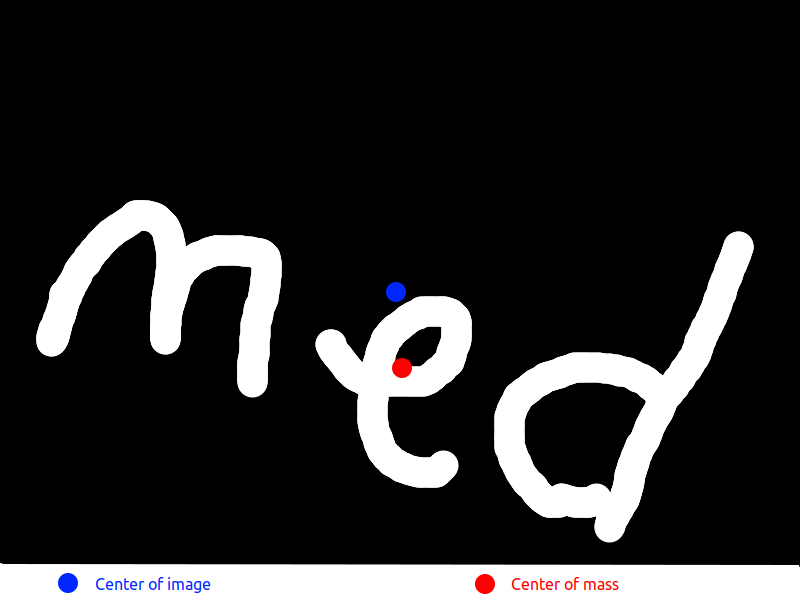
\includegraphics[width=0.6\textwidth]{mep_img/center_of_mass.png}
\caption{Trọng tâm của một hình ảnh còn dựa vào khôi lượng tại mỗi điểm ảnh bên trong.}\label{center_of_mass}
\end{figure}

Sau khi có công thức tính toán khoảng cách giữa 2 node, ta sẽ tiếp tục sử dụng Average-Linkage để tính toán khoảng cách giữa 2 cụm với nhau. Average-Linkage sẽ tính toán trung bình khoảng cách từ mỗi bounding box từ cụm này tới các node tương ứng trong cụm bên kia theo công thức trong ~\ref{eq:Average_Linkage}.

\begin{dmath}
    \label{eq:Average_Linkage}
    \text{DIST_AVG(} {\{x_n\}}_{n=1}^N, {\{y_m\}}_{m=1}^M \text{)} = \frac{1}{NM}\sum_{n=1}^{N}\sum_{m=1}^{M} ||x_n - y_m ||
\end{dmath}

Để đảm bảo gom cụm đạt hiệu quả về cả thời gian cũng như chất lượng, chúng tôi thực hiện nâng cấp bằng cách cắt tỉa thuật toán thông qua một ngưỡng threshold. Threshold này yêu cầu khoảng cách giữa 2 cụm không được lớn hơn, dẫn đến hệ quả là 2 bounding box không thuộc cùng một dòng sẽ không bao giờ phải gom lại thành một cụm, đồng thời kết thúc sớm thuật toán và trả ra kết quả. MergeOCR được thực hiện sau khi nhận dạng văn bản bằng OCR, cho nên các bounding box nằm trên 1 dòng vẫn được nhận dạng riêng biệt, và giúp cho việc nhận dạng của VietOCR đạt hiệu quả hơn, tránh bị nhiễu.

Thuật toán ~\ref{alg:AHC} mô tả chi tiết phiên bản AHC do chúng tôi đề xuất và tối ưu, dựa trên thuật toán gốc tại \cite{day1984efficient}.

\begin{algorithm}[H]
    \caption{Agglomerative Hierarchical Clustering} \label{alg:AHC}
    \begin{algorithmic}[1]
        \State \textbf{Input: } Vector trọng tâm của các bounding box $\{ x_n \}_{n=1}^{N}$, ma trận khoảng cách giữa các cluster $DIST(G_1, G_2)$ tương ứng.
        \State \textbf{Input 2: } $\varepsilon \ gets threshold$ \Comment{Threshold quy định ngưỡng để coi 2 input nằm trên cùng dòng.}
        \State Khởi tạo $A \gets \emptyset$.
        \For{$n \gets 1...N $}
            \State $A \gets A \cup \{\{x_n\}\}$ \Comment{Khởi tạo mỗi nhóm sẽ chứa một bounding box}
        \EndFor
        
        \State $T \gets A$ \Comment{Khởi tạo cây lưu kết quả merge.}
        \State $D_{min} = +\infty$ \Comment{khởi tạo khoảng cách nhỏ nhất giữa hai input.}
        
        \While{$|A| > 1$ \textbf{and} $D_{min} > \varepsilon$} \Comment{Lặp cho đến khi tập A chỉ còn 1 phần tử hoặc không merge được nữa do không thỏa ngưỡng.}
                \State $G_1^{*}, G_2^{*} \gets \argmin_{G_1, G_2 \in A; G_1, G_2 \in A}$ $DIST(G_1, G_2)$ \Comment{Tìm ra cặp cluster cũ gần nhau nhất.}
                
                \State $A \gets (A \setminus \{ G_1^* \}) \setminus \{ G_2^* \}$ \Comment{Loại cặp cluster cũ ra khỏi tập tìm input.}
                
                \State $A \gets A \cup \{ G_1^* \cup G_2^* \}$ \Comment{Lưu tập mới tìm được vào tập input.}
                
                \State $T \gets T \cup \{ G_1^* \cup G_2^* \}$ \Comment{Lưu tập mới tìm được vào cây kết quả.}
                
                \State $D_{min} \gets DIST(G_1^*, G_2^*)$ \Comment{Gán lại khoảng cách nhỏ nhất}
        \EndWhile
        
        \State \textbf{Return: } $T$. \Comment{Trả về kết quả các cụm là các dòng trong văn bản.}
        
    \end{algorithmic}
\end{algorithm}

Kết quả của bước này sẽ là nhiều cụm, mỗi cụm có chữa nhiều bounding box, từ đây các văn bản trong cùng một cụm, hay nói cách khác là trên cùng một dòng, sẽ được nối với nhau theo thứ tự từ trái sang phải theo trục X. Văn bản này đáp ứng tốt yêu cầu đầu vào của Medicine Extractor như trong hình ~\ref{merged_img}, từ đó cải thiện toàn bộ hệ thống \codeword{MEP} của chúng tôi.

\begin{figure}
\centering
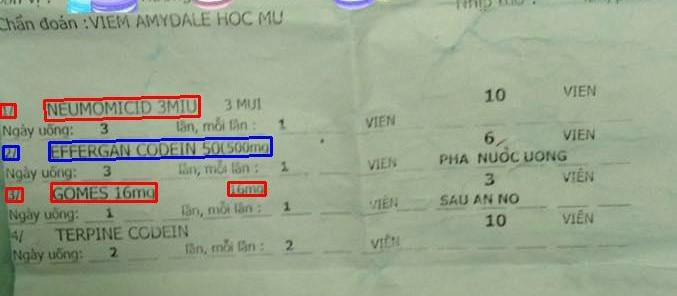
\includegraphics[width=0.7\textwidth]{mep_img/merged_img.png}
\caption{MergeOCR giúp gộp các bounding box trên một dòng lại với nhau.}\label{merged_img}
\end{figure}

\section{Medicine Classifier}

Với sự hỗ trợ từ MergeOCR và Medicine Extractor, ta đã có thể lấy được các tên thuốc tiềm năng, và nhiệm vụ tiếp theo chính là lấy được chính xác tên thuốc trên dòng chứa tên thuốc đó. Thông thường, một dòng chứa tên thuốc có thể chứa nhiều thành phần, bao gồm số thứ tự, tên thuốc, hoạt chất, liều lượng, cách dùng, chỉ định... Đặc biệt, dù đa số đơn thuốc đều có mẫu cố định là có số thứ tự, tuy nhiên về thứ tự giữa tên thuốc và hoạt chất thì lại không có một chuẩn chung. Tên thuốc có thể đứng trước hoạt chất, hoặc ngược lại, thậm chí có trường hợp đơn thuốc không có hoạt chất trong dòng đó. 

Như vậy, cần có một mô hình giúp phân lớp xem một đoạn văn bản có phải là tên thuốc hay không, đồng thời giảm thời gian xử lý toàn bộ dữ liệu đầu vào và giải quyết bài toán một cách chính xác hơn. Đây chính là bài toán phân lớp văn bản (Text Classification) trong lĩnh vực xử lý ngôn ngữ tự nhiên (NLP). Dựa trên ưu điểm đã phân tích của mô hình TCN, chúng tôi sử dụng nó cho \codeword{MEP}, đặt tên là Medicine Classifier, có kiến trúc được mô tả trong hình ~\ref{medicine_classifier_1}.

\begin{figure}
\centering
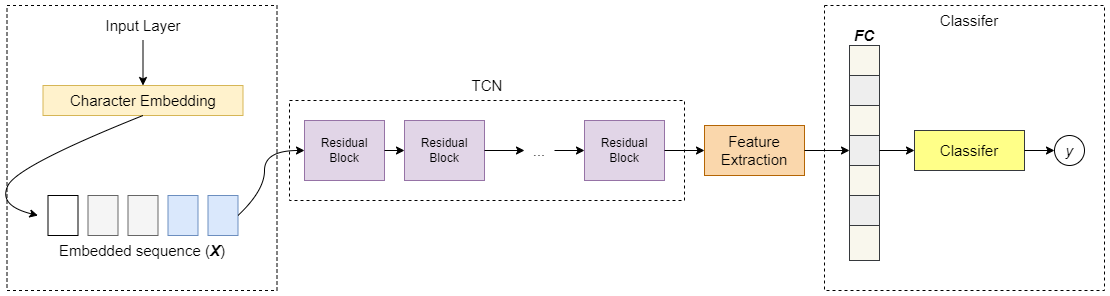
\includegraphics[width=1.0\textwidth]{mep_img/medicine_classifier_1.png}
\caption{Mô hình Medicine Classifier do chúng tôi đề xuất nhằm phân lớp văn bản.}\label{medicine_classifier_1}
\end{figure}

Cấu trúc mô hình bao gồm 2 phần chính, cụ thể như sau. Phần đầu tiên, văn bản đầu vào sẽ được đẩy qua bộ character embedding để chuyển về một chuỗi giá trị (sequence). Sau đó thông qua việc padding với câu dài nhất tại thời điểm huấn luyện nhằm giúp các câu khác nhau đều được biểu diễn về cùng một kích thước. Các giải pháp cho bài toán phân lớp văn thường được ứng dụng cho việc phân lớp nguyên một câu hay cả đoạn văn, bài văn. Vì thế, thông thường người ta hay dùng word embedding để giúp cho mô hình học được ngữ cảnh của văn bản tốt hơn thông qua sự liên kết giữa các từ trong câu. 

Tuy nhiên, đối với tên thuốc, nó thuộc dạng short-text, chỉ cấu tạo từ một đến một vài từ là tối đa. Tên thuốc thường được cấu tạo từ một số các kí tự mà khi ghép lại với nhau thì tỏ ra vô nghĩa, không giống với cách cấu trúc của từ ngữ thông thường. Vì vậy, chúng tôi đề xuất sử dụng character embedding để thay thế cho word embedding. Cách này vừa có thể khắc phục vấn đề , vừa có thể xử lý cả các tên thuốc bị sai cú pháp (misspelling). Thêm nữa, khi dùng character embedding, ta có thể có được một sequence đủ dài đối với cả short-text, từ đó hạn chế được overfitting.

Phần thứ hai là mô hình TCN. Nó giúp ta học được sự liên kết giữa các ký tự trong sequence của character embedding.Việc bị thiếu hay bị sai một kí tự sẽ không ảnh hưởng nhiều đến tổng thể của chuỗi, do vậy nó vẫn đảm bảo hoạt động tốt ngay cả khi tên thuốc bị đánh sai cú pháp. Đồng thời, hiệu năng của TCN đạt được khá tốt. Nó có thể xử lý một lượng lớn input trong một thời gian ngắn. Các feature sau khi qua TCN sẽ được đẩy đến lớp fully connected, với mục tiêu là phân thành 3 lớp cố định. Cụ thể, ta sẽ phân lớp ra thành tên thuốc, hoạt chất và unknown (tức là không thuộc 2 lớp tên thuốc hoặc hoạt chất).

Dữ liệu huấn luyện của Medicine Classifier bao gồm, tên thuốc và hoạt chất được tách riêng từ từ điển thuốc, còn các tên tự do được thu thập từ dữ liệu hỏi đáp trên Yahoo. Tất cả các nhóm input đều được lọc và làm sạch để sao cho có cùng đặc trưng, như là min, mean, median, std, max. Đồng thời, để đảm bảo tất cả đều là short-text, chúng tôi cũng giới hạn số từ trong mỗi input không vượt quá một ngưỡng nhất định là 5 từ, cũng là số từ tối đa của tập dữ liệu các tên thuốc phổ biến. 

Đầu ra của mô hình Medicine Classifier cho mỗi nhãn input chính là một chuỗi các xác suất để phân văn bản đó vào lớp tương ứng. Mô hình sẽ quy định một ngưỡng threshold nhất định để xác định xem nhãn đó gần với lớp nào nhất. Với việc đảm bảo chất lượng của dữ liệu huấn luyện, chúng tôi kì vọng mô hình Medicine Classifier sẽ hoạt động hiệu quả nhằm phân loại chính xác đâu là tên thuốc, đâu là hoạt chất, và loại ra những tên không hợp lệ trước khi tiếp tục đưa vào bước sau.

\section{Context Aware spell correction}

Sau khi đã thực hiện bước Medicine Classifier, ta đã bỏ những dòng nào không chứa các cụm văn bản được phân lớp vào tên thuốc hoặc hoạt chất. Càng ít dòng được giữ lại, thời gian xử lý sẽ càng được rút ngắn, giúp tối ưu hiệu năng cho toàn bộ hệ thống. Tuy nhiên, bởi vì vẫn có sự nhập nhằng giữa tên thuốc và hoạt chất. Như đã đề cập, đôi khi tên thuốc cũng là hoạt chất, và ngược lại. Cụ thể, đôi khi một dòng vừa chứa tên thuốc và hoạt chất, nhưng hệ thống Medicine Classifier có thể phân cả 2 thành tên thuốc, hoặc cả 2 thành hoạt chất. Vì thế, bước cuối cùng này mục tiêu để lọc bỏ, chỉ giữ lại một tên có khả năng cao là tên thuốc nhất.

Bằng cách so sánh mỗi tên với một bộ từ điển được giới hạn trong phạm vi tên thuốc. Chúng tôi thực hiện tìm kiếm mờ dựa trên khoảng cách Levenshtein (Levenshtein Distance \cite{Levenshtein_distance}) nhằm tối ưu chi phí tính toán. Các tên thuốc sẽ được tìm kiếm gần đúng với tên thuốc gần nhất trong bộ từ điển. Công thức tính khoảng cách Levenshtein được mô tả chi tiết trong hình ~\ref{lev_dist}.

\begin{figure}
\centering
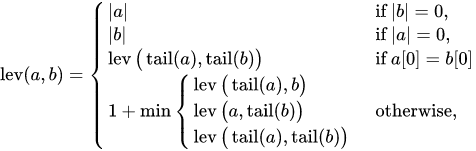
\includegraphics[width=0.7\textwidth]{mep_img/lev_dist.png}
\caption{Công thức tính khoảng cách Levenshtein Distance \cite{Levenshtein_distance}.}\label{lev_dist}
\end{figure}

Về cách cài đặt thuật toán, chúng tôi thực hiện thủ thuật cache lại kết quả cũ để tăng tốc độ tìm kiếm. Chúng tôi chia tập từ điển đơn thuốc ra thành hai, trong đó tập đầu tiên là tập từ điển gốc với kích thước lớn. Khi thực hiện tìm kiếm mờ trên tập này sẽ tốn một lượng thời gian đáng kể. Chính vì vậy chúng tôi sẽ lưu trữ thêm một tập thứ 2 có kích thước nhỏ, chỉ chứa những thuốc thường xuyên được sử dụng bởi hệ thống. Vì tập này có kích thước nhỏ hơn hẳn nên thời gian truy vấn sẽ rất tối ưu, gần như ngay lập tức trả ra kết quả khi có yêu cầu. Hình ~\ref{med_recorrected} chỉ ra một kết quả của đơn thuốc sau khi được trích xuất và sửa lỗi tên thuốc theo như trong từ điển.

\begin{figure}
\centering
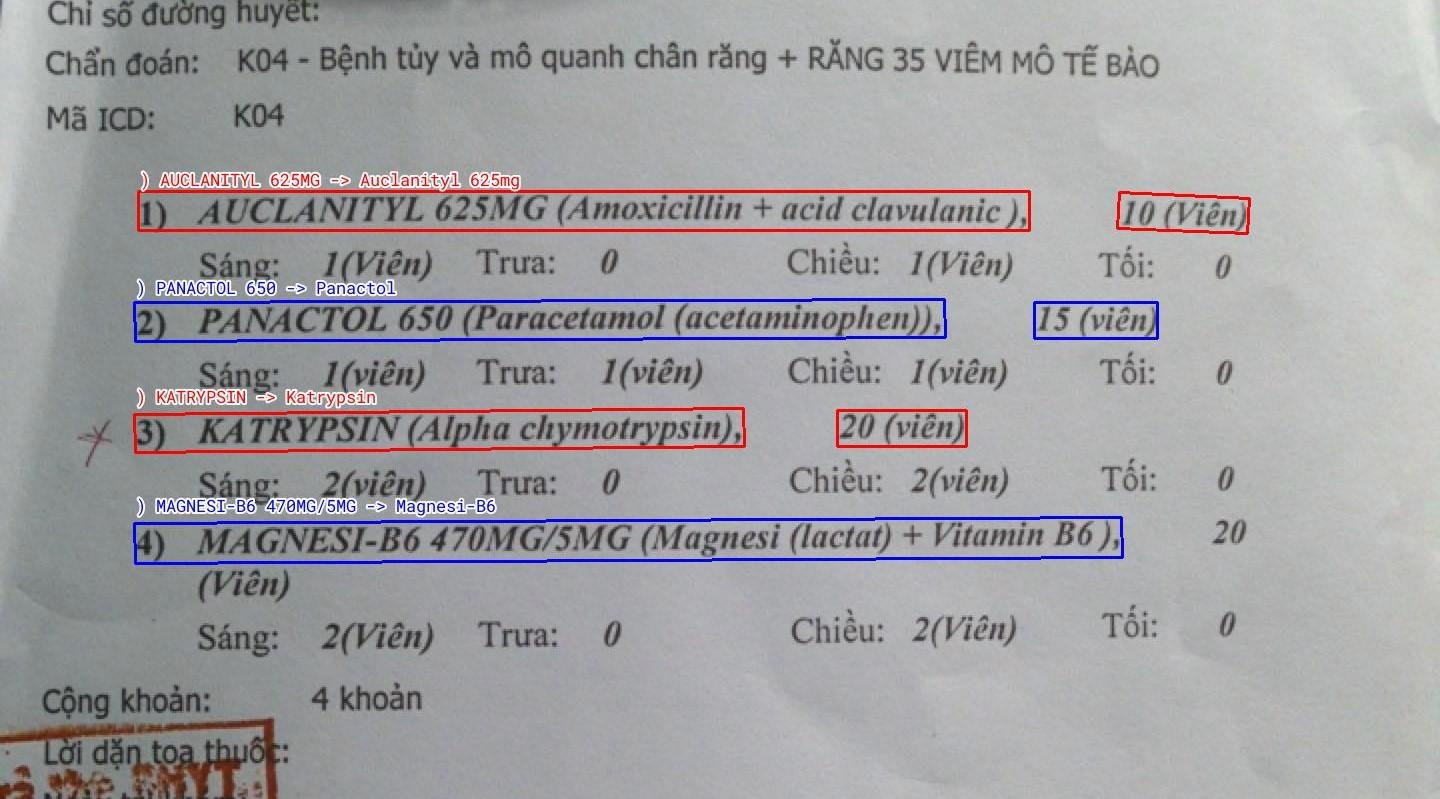
\includegraphics[width=0.7\textwidth]{mep_img/med_recorrected.png}
\caption{Đơn thuốc sau khi trích xuất thông tin tên thuốc và sửa lỗi.}\label{med_recorrected}
\end{figure}